In order to have a better idea of the performances of the DBC regarding the bandwidth of the signal, simulation of the retrieved visibilities and phases have been ran. To do that the simulated polychromatic light is injected into 2 of the 4 inputs. At one of the input a phase is added just the same as for constructing the V2PM. At each output an interferogram is reconstructed showing the visibility function versus the OPD. These interferogram (in the shape of a matrix where each column is one simulated phase of the \gls{bl}) are multiplied by the P2VM to obtain the $\vec{V}$ vector from which the object visibility are calculated as explained in sections \ref{sec:mathmono} and \ref{sec:mathpoly}. The results are presented in Fig.\ref{fig:retrieved_nofan} and Fig.\ref{fig:retrieved_fan}

In our simulation no polarization's effects are taken into account so that the visibility of the input source should be 1 at the 0 OPD independently of the phase difference. All simulations were performed with one data point each 12 degrees of phase difference between the inputs from 0 to 360 degrees, for all 50 wavelength evenly spaced in a fixed bandwidth around 3.4 µm and for all 6 baselines. 

To estimate the accuracy of the retrieved phases and visibilities, the expected ones are subtracted from the retrieved ones and the deviation $\epsilon$ is estimated by the formula :
\begin{equation}\label{eq:deviation}
\epsilon = \sqrt{\frac{1}{N}\sum_{1}^{N}(a-\Tilde{a})^2}
\end{equation}

where $a$ is the retrieved parameters, $\Tilde{a}$ the expected one and $N$ the number of tested retrieved parameters (31 in out case).
The result is shown in Fig \ref{fig:retrieved_nofan}. What can be seen is that the retrieved visibilities are close to the expected ones (at $\pm5\%$ for bandwidth below 60 nm bandwidth), same as the retrieved phases (at $\pm 0.05 rad$ below 60 nm bandwidth).
Meanwhile the standard deviation of both the retrieved phases and visibilities are found to have a similar dependency to the bandwidth. This means that the larger the bandwidth, the more dispersed the retrieved parameters around their mean value. 
The results for the component with a "fan-out" is very similar as can be seen in Fig. \ref{fig:retrieved_fan} despite a lower condition number of the V2PM. This clearly shows that the condition number only states the maximum magnification of an error. It also shows that despite the apparent correlation between the retrieved visibilities/phases and the condition number of the V2PM, the impact of this condition number is not the main limiting factor but the approximations of "flat spectral response" is. The broader the bandwidth the more the spatial frequency of the interferogram (i.e the fringe spacing) can get different from 3.4 \si{\micro\meter} leading to errors on both the retrieved phase and visibility. 


\begin{figure}[htbp]
    \centering
    \begin{subfigure}{.45\textwidth}
        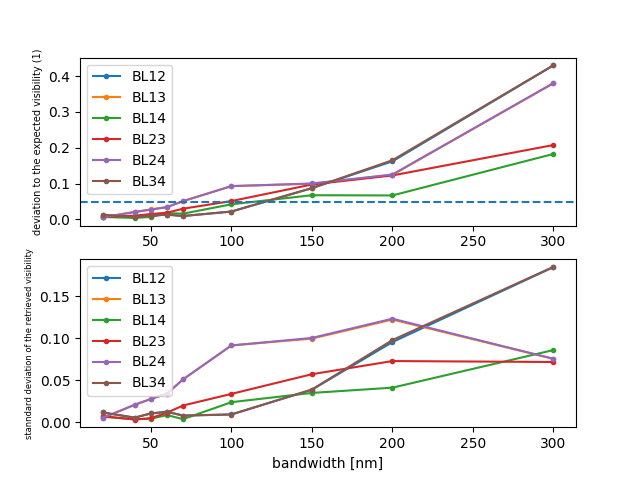
\includegraphics[scale=.45]{picture/retrieval_simu/visi_retrieved_nofan.png}
        \caption{Deviation of the retrieved visibilities to the expected ones}
    \end{subfigure}%
    \begin{subfigure}{.45\textwidth}
    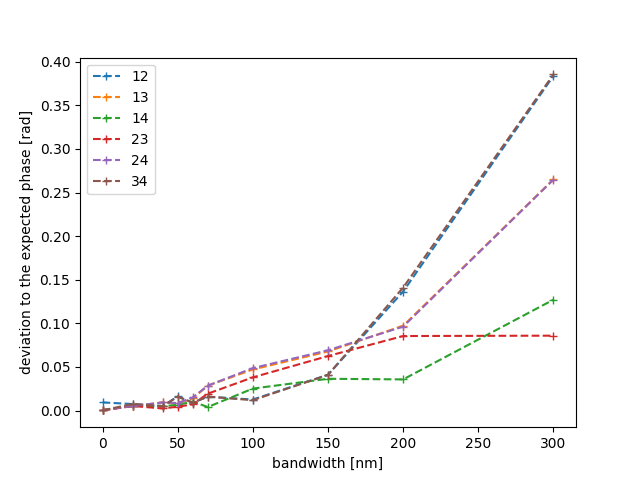
\includegraphics[scale=.45]{picture/retrieval_simu/phase_retrieved_nofan.png}
    \caption{Deviation of the retrieved phases to the expected ones}
    \end{subfigure}
    \caption{Deviation of the retrieved phases and visibilities to the expected ones for the component without fan-out. The deviation is calculated by Eq. \ref{eq:deviation}}. In order to compare with the experimental results presented in the following part, the plots of the retrieved visibility and phases with 70nm bandwidth are presented in Appendix \ref{an:retriev}. The retrieving algorithm show good accuracy for a bandwidth below 70nm and for each baselines individually. But the component is designed to be used with the 4 input beams at the same time. The next part will present the results of simulations using the 4 beams at the same time.   
    \label{fig:retrieved_nofan}
\end{figure}

\begin{figure}[htbp]
    \centering
    \begin{subfigure}{.45\textwidth}
        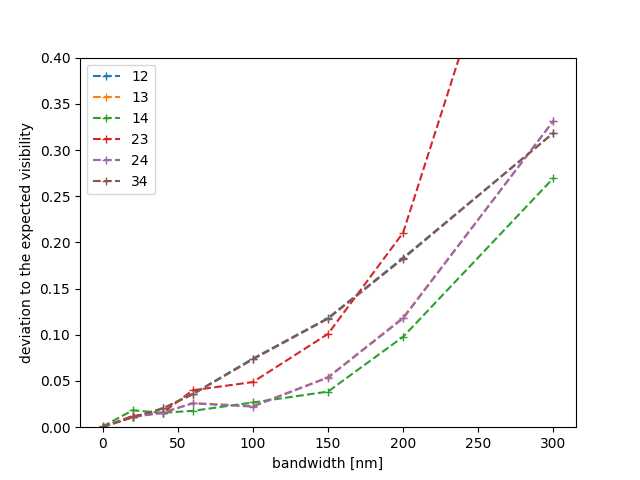
\includegraphics[scale=.45]{picture/retrieval_simu/visi_retrieved_fan.png}
        \caption{Standard deviation  of the retrieved visibilities to the expected ones}
    \end{subfigure}%
    \begin{subfigure}{.45\textwidth}
    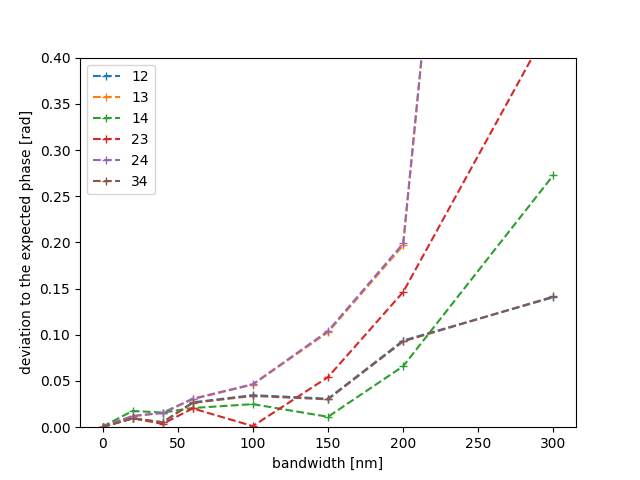
\includegraphics[scale=.45]{picture/retrieval_simu/phase_retrieved_fan.png}
    \caption{Standard deviation of the retrieved phases to the expected ones}
    \end{subfigure}
    \caption{Standatd deviation of the retrieved phases and visibilities to the expected ones for the component with fan-out. The deviation is calculated by Eq. \ref{eq:deviation}. The blue dashed line is the limit of 5\% error. Inputs 1,2,3,4 refers respectively to WG 19,14,10,5 in Fig.\ref{tikz:ZigZagCrossSection} as seen from the inputs.}
    \label{fig:retrieved_fan}
\end{figure}

\subsubsection{Retrieved visibility and phase using the 4 input beams}
To this point only retrieved visibility and phases using 2 beams at a time have been presented. The component being designed to combine 4 telescopes at the same time, simulation doing that have been done. to this purpose the previously calibrated P2VM are used and applied to the results of a simulation using the 4 input. The phase of three beams have been fixed and the phase of the last beam has been scanned to simulate the behaviour of the component. Only one test have been done using at $\lambda_0=3.4 \mu m$ and 20nm bandwidth. 

First the component \emph{without fanout} has been simulated. The results are shown in Fig.\ref{fig:4BL_sim_nofan} and Fig.\ref{fig:4BL_sim_nofan_phase}. The retrieved visibility are far less accurate when using 4 beams at the same time than when using only 2 beams at the same time (error up to 25\%). The reason to that is the combination of the previously exposed "apparent wavelength" of the interferograms and the fact that in those simulations the "0 OPD" (i.e the maximum of each interferogram) appears for all baselines at approximately the same OPD. Therfore each baselines are less distinguishable from each-other, a phase shift between each of the 6 baselines would probably lead to better results, this would be a thing to try in order to confirm or invalidate this interpretation.
Concerning the retrieved phase, the accuracy is relatively good (lower than 0.12 rad of error). Still the error is two times the ones obtained when using two beams at a time. The explanation of this is the same than for the visibility.

\begin{figure}[htbp!]
\centering
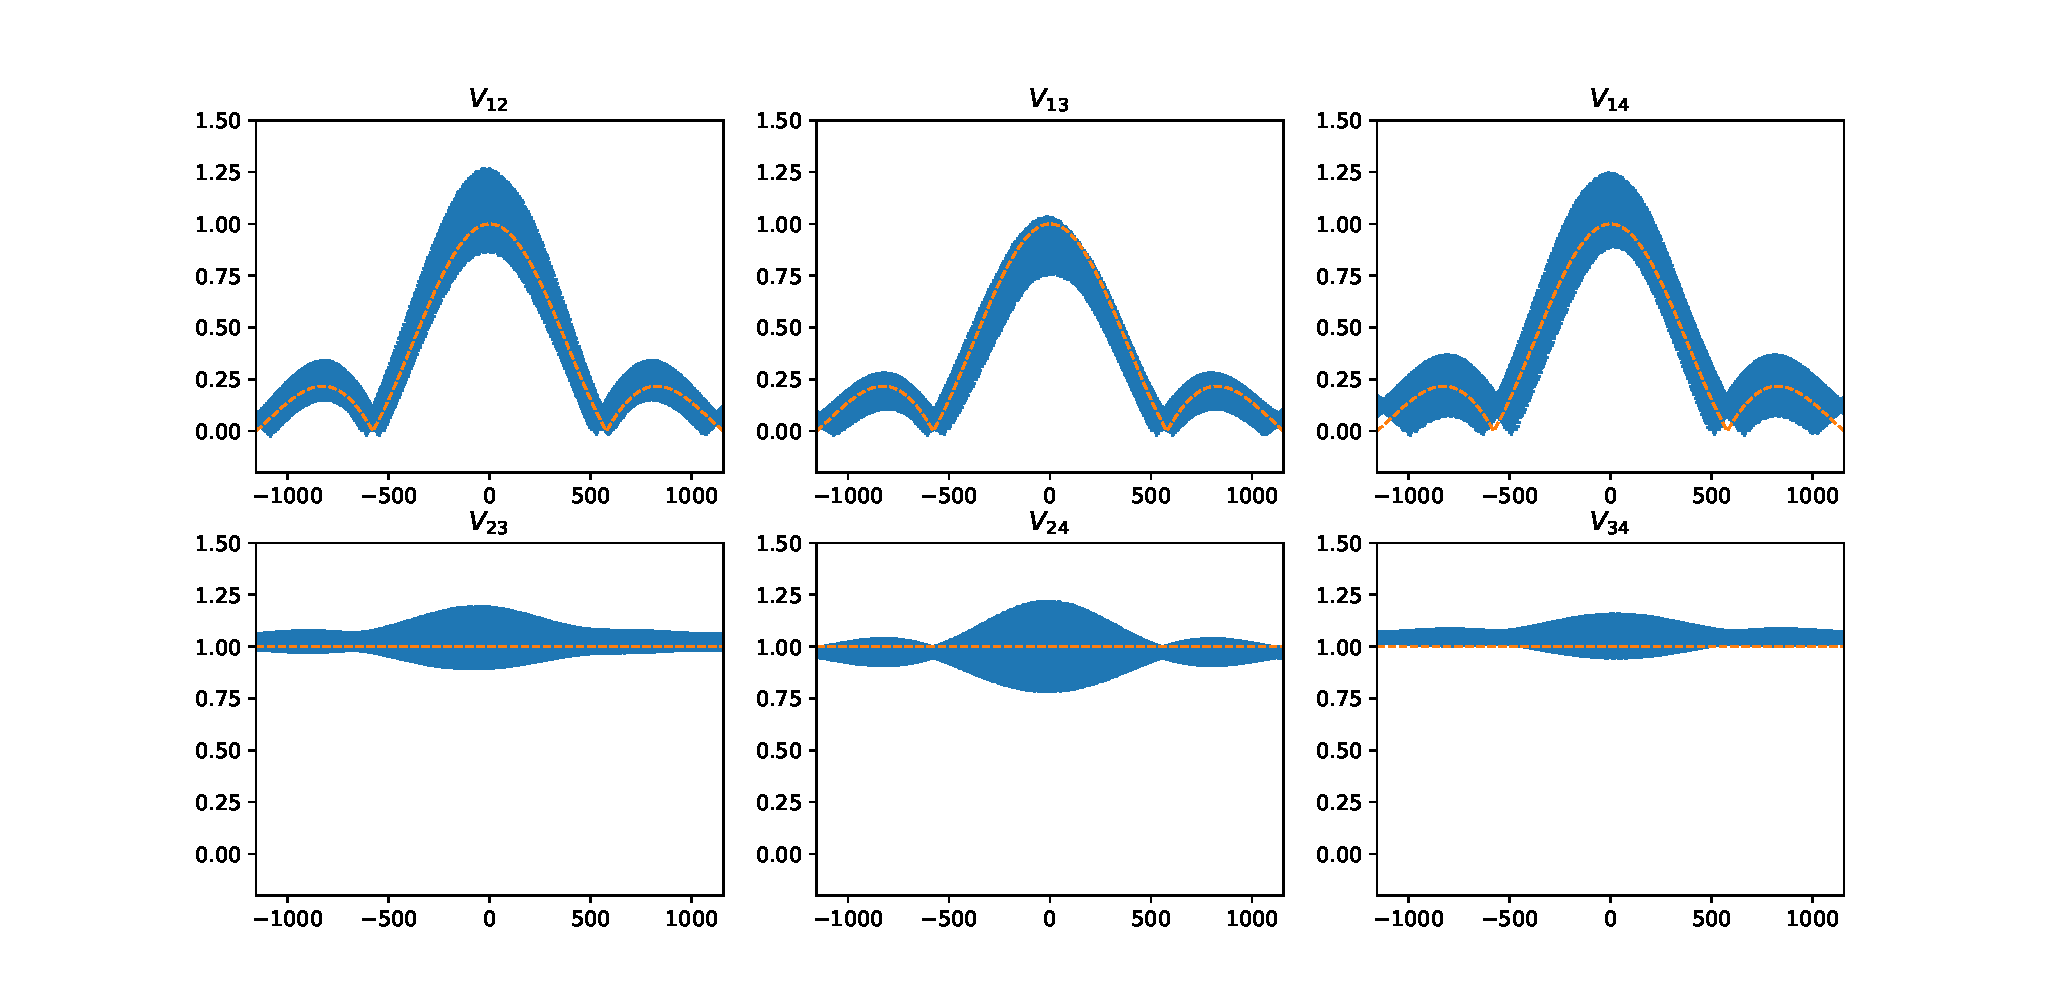
\includegraphics[scale=.4]{../picture/4BL_20_nofan.pdf}
\caption{Simulated retrieved visibility using the 4 beams on the component without fanout. The signal bandwidth used is 20nm centred at $ \lambda_0=3.4 \mu m$. The blue line is the retrieved date. The orange dotted line is the expected one. The x-axis is the OPD in µm and the y-axis the visibility.}
\label{fig:4BL_sim_nofan}
\end{figure}


\begin{figure}[htbp!]
\centering
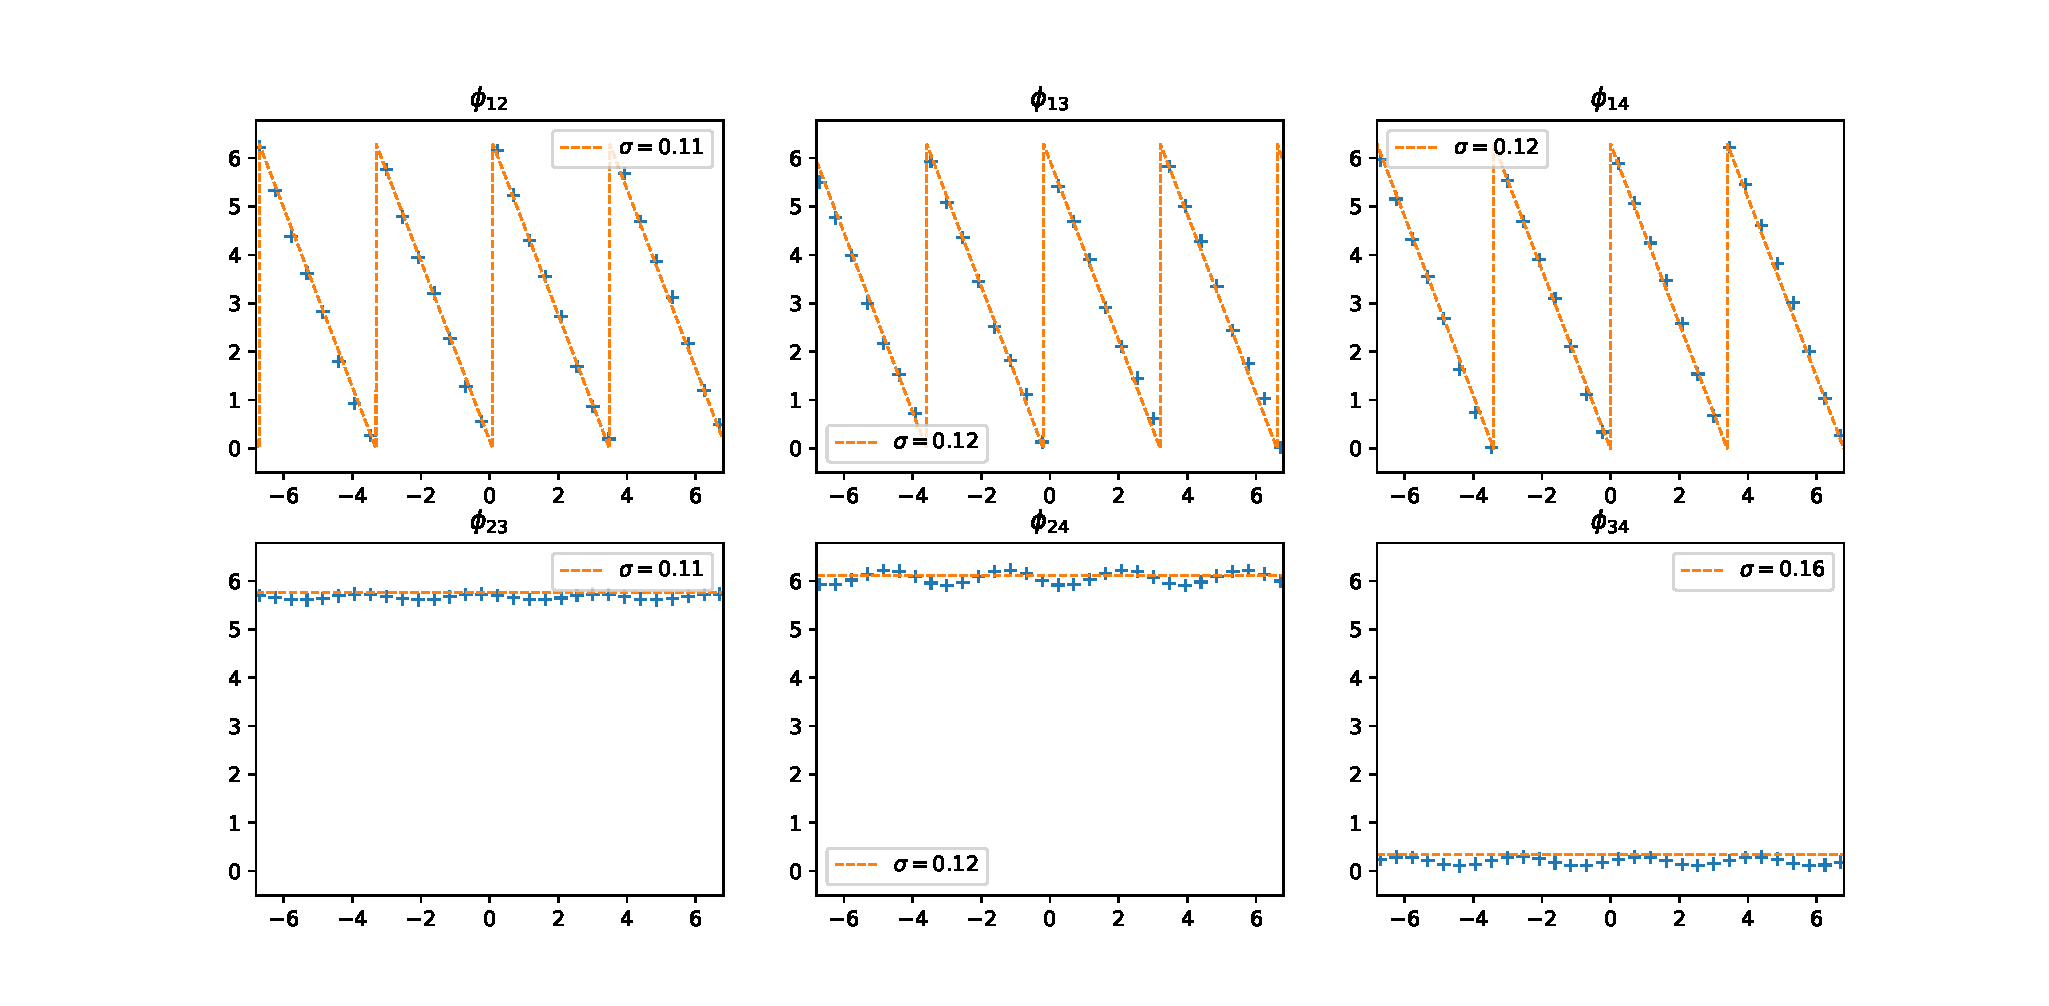
\includegraphics[scale=.4]{../picture/4BL_20_nofan_phase.pdf}
\caption{Simulated retrieved phase using the 4 beams on the component without fanout. The signal bandwidth used is 20nm centered at $ \lambda_0=3.4 \mu m$. The blue line is the retrieved date. The orange dotted line is the expected one. The x-axis is the OPD in µm and the y-axis the phase in rad. Sigma is the standard deviation to the expected phase in rad.}
\label{fig:4BL_sim_nofan_phase}
\end{figure}

Secondly the component \emph{with fanout} has been simulated. The results are shown in Fig.\ref{fig:4BL_sim_fan} and Fig.\ref{fig:4BL_sim_fan_phase}. In that both the errors on the retrieved phase and visibility are good and comparable to the ones obtained using two beams at a time (visibility at $\pm 5\%$ and phase at $\pm 0.08 rad$). The explanation to this could be that the "fan-out" lead to "0 OPD" of each output being further to each other and for each baselines too. More simulations should be done with this component in order to confirm or invalidate that interpretation.  

\begin{figure}[htbp!]
\centering
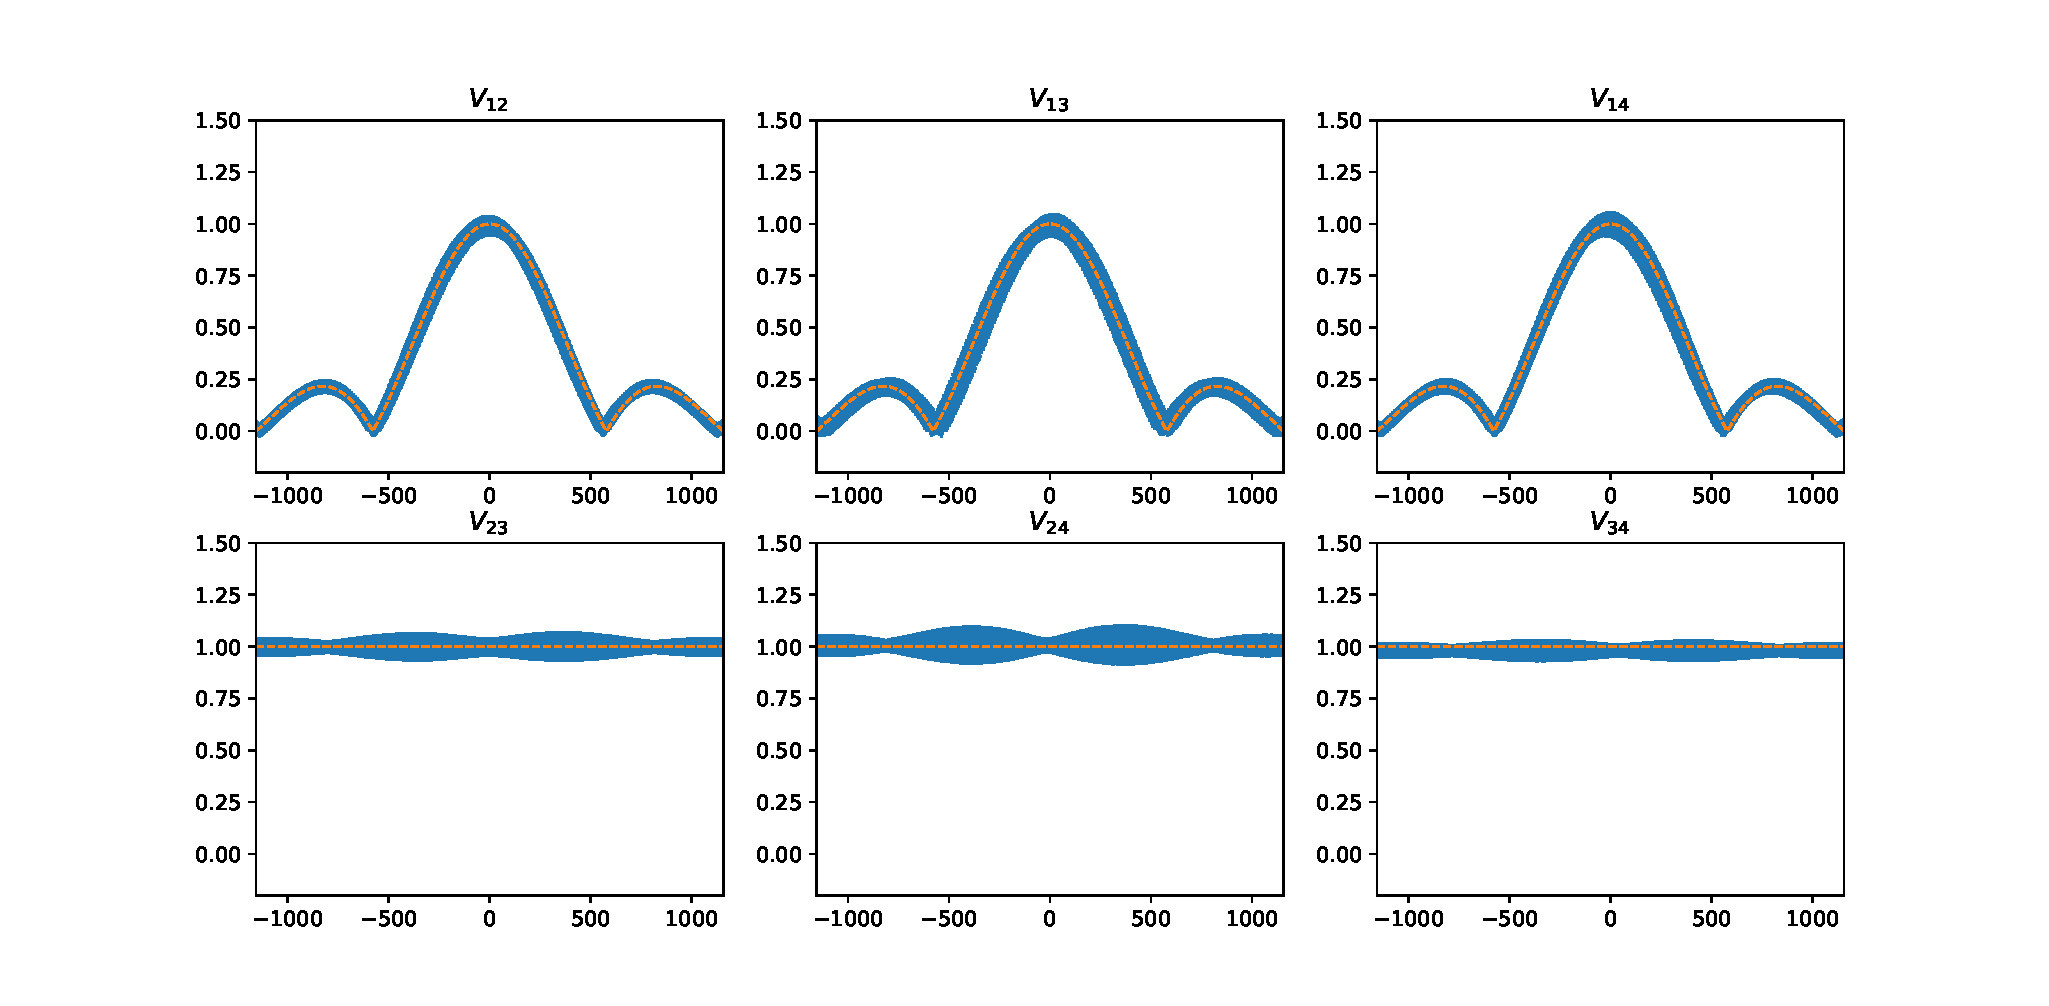
\includegraphics[scale=.4]{../picture/4BL_20_fan.pdf}
\caption{Simulated retrieved visibility using the 4 beams on the component with fanout. The signal bandwidth used is 20nm centred at $ \lambda_0=3.4 \mu m$. The blue line is the retrieved date. The orange dotted line is the expected one. The x-axis is the OPD in µm and the y-axis the visibility.}
\label{fig:4BL_sim_fan}
\end{figure}


\begin{figure}[htbp!]
\centering
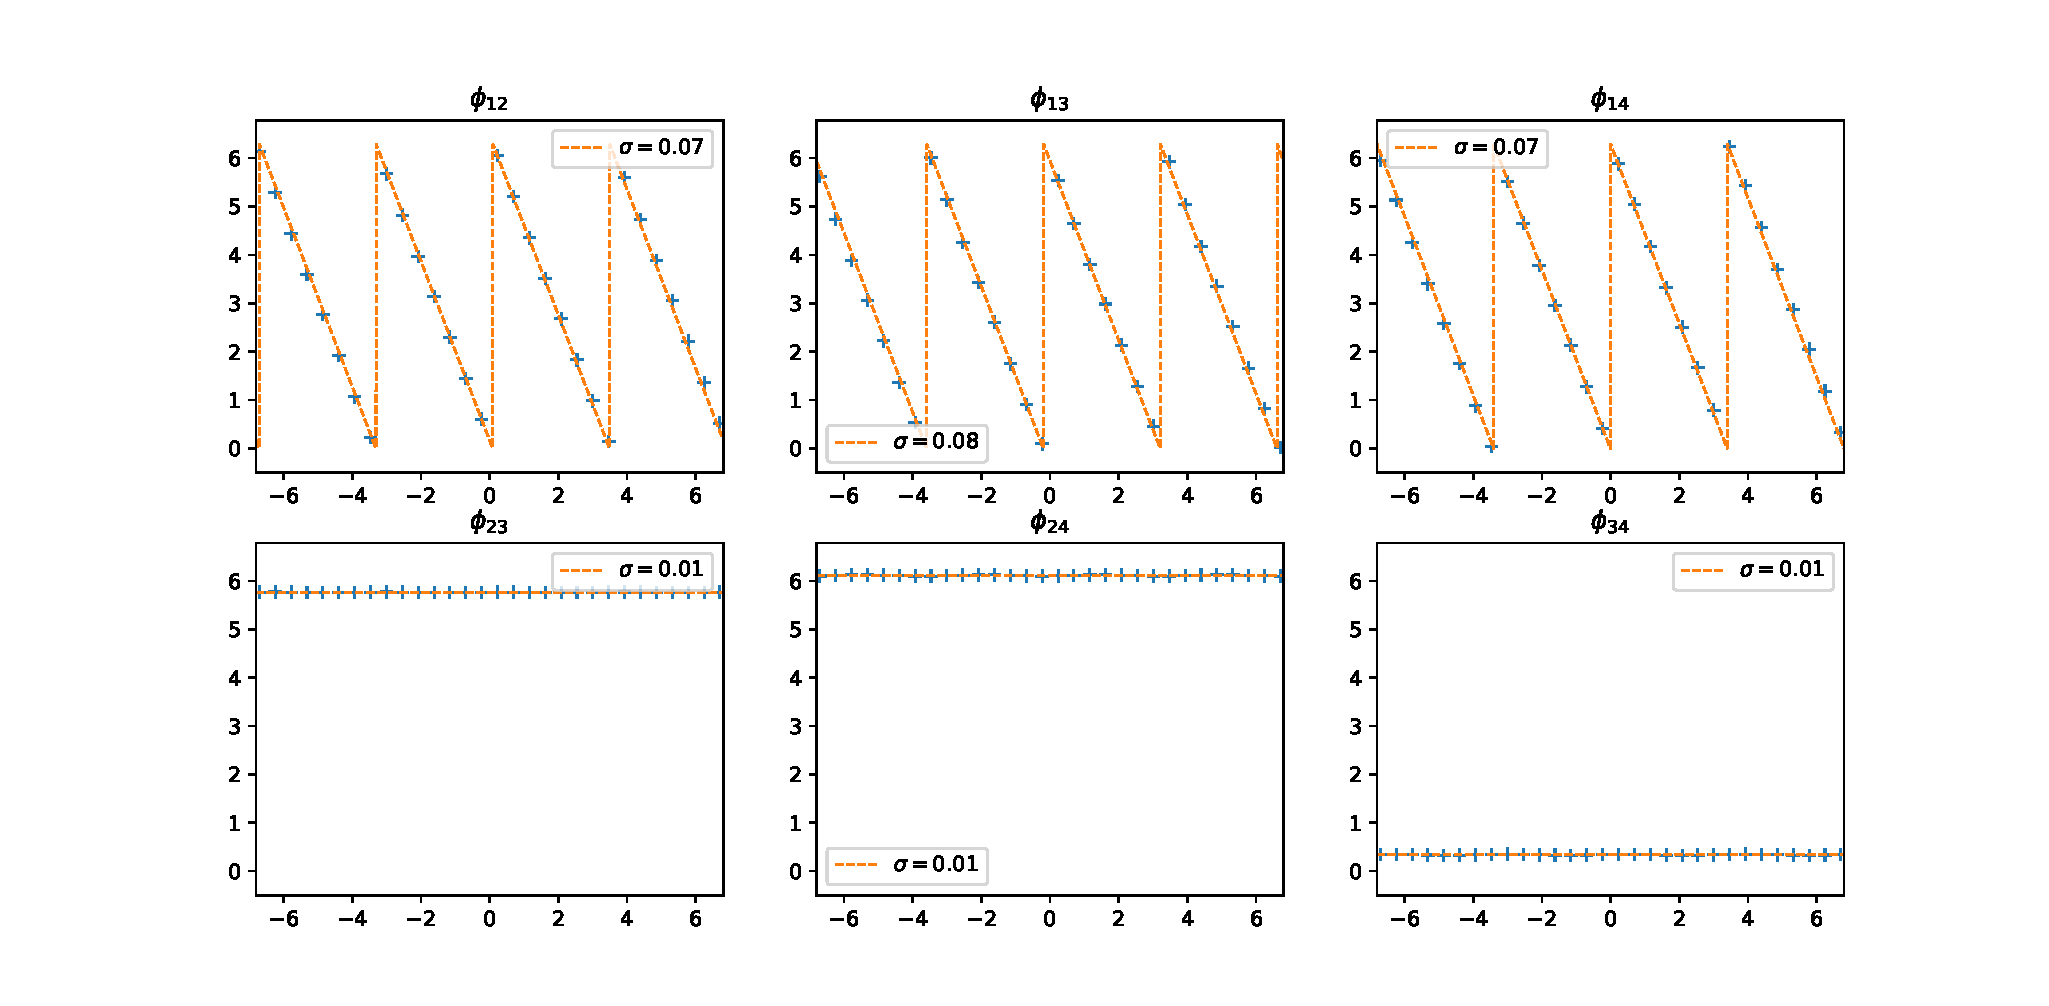
\includegraphics[scale=.4]{../picture/4BL_20_fan_phase.pdf}
\caption{Simulated retrieved phase using the 4 beams on the component with fanout. The signal bandwidth used is 20nm centered at $ \lambda_0=3.4 \mu m$. The blue line is the retrieved date. The orange dotted line is the expected one. The x-axis is the OPD in µm and the y-axis the phase in rad. Sigma is the standard deviation to the expected phase in rad.}
\label{fig:4BL_sim_fan_phase}
\end{figure}



The results of these simulations enlighten that the component with fanout could have better performances when used with 4 beams under the exact same conditions than the component without fanout. This difference is expected to be even greater experimentally due to the previously exposed problem of the integrating area. In simulation accuracy of 5\% on the retrieved visibility and 0.08 rad on the retrieved phases have been obtained using the 4 inputs at the same time with the component with "fanout" and a signal's spectral bandwidth of 20nm. When using 2 beams at the same time, a spectral bandwidth of 70nm led to an acceptable simulated accuracy on the retrieved parameters. 
An experimental demonstration of the usability of the DBC with a signal of 70nm bandwidth (limit of acceptable accuracy using two beams at a time) is still to be done. This is the purpose of the next chapter.
